\subsection{Distributed Checkpoint}

Traditional checkpointing tightly couples saved model state with the specific parallelism configuration, requiring complex offline conversion when changing TP, EP, PP, or other parallelism settings. Our distributed checkpoint library solves this through \textbf{parallelism-agnostic checkpointing} with automatic resharding.

The core abstraction is the \texttt{ShardedTensor} descriptor, which encodes each local tensor's global shape, offset, and sharding pattern. During saving, each rank independently writes its local shard (Fully Parallel Saving), eliminating coordinator bottlenecks. During loading, each rank determines which portions of global tensors it needs based on the \textit{new} sharding specification and reads only those slices.

This enables any-to-any parallelism reconfiguration: a checkpoint saved with $\text{TP}=2$, $\text{EP}=4$ can be loaded with $\text{TP}=4$, $\text{EP}=8$ without offline conversion. The library supports Zarr (default) and PyTorch Distributed~\cite{zhao2023pytorchfsdp} storage backends.

\subsection{Flexible Asymmetric Virtual Pipeline Parallelism}\label{sec:flexible-vpp}

Interleaved pipeline parallelism~\cite{narayanan2021efficient} divides each physical pipeline stage into multiple virtual stages with interleaved scheduling, mitigating pipeline bubbles. Traditional VPP requires uniform layer distribution (e.g., a 24-layer model with $\text{PP}=4$, $\text{VPP}=2$ distributes layers as $[6, 6, 6, 6]$). However, MoE models exhibit substantial workload heterogeneity: MoE layers, dense layers, embedding, loss, and specialized layers like MTP have significantly different computational costs.

We introduce \textbf{Flexible Asymmetric VPP}, which allows different numbers and types of layers per virtual stage. Consider DeepSeek-V3 with 61 decoder layers and 1 MTP layer at $\text{PP}=16$, $\text{VPP}=2$ (Table~\ref{tab:flexible-vpp-example}). The initial rank combines the lightweight embedding with 3 dense decoders (matching the cost of 2 MoE layers). Most ranks hold 2 MoE decoders per stage. The final ranks strategically place the heavy MTP layer and lightweight loss layer to balance workload.

This approach enables VPP for models with arbitrary layer counts, achieves true load balancing by accounting for per-layer computational costs, and provides flexible placement for specialized layers.

\begin{table}[ht]
\centering
\caption{Layer distribution for DeepSeek-V3 with flexible asymmetric VPP ($\text{PP}=16$, $\text{VPP}=2$).}
\label{tab:flexible-vpp-example}
\begin{tabular}{lll}
\toprule
\textbf{PP rank} & \textbf{VPP rank 0} & \textbf{VPP rank 1} \\
\midrule
0       & embedding + 3$\times$ decoder & 2$\times$ decoder \\
1--13   & 2$\times$ decoder             & 2$\times$ decoder \\
14      & 2$\times$ decoder             & MTP \\
15      & 2$\times$ decoder             & loss \\
\bottomrule
\end{tabular}
\end{table}

This flexible asymmetric approach (\figref{fig:flexible-vpp-layout}) delivers several key advantages: (1) it enables VPP for models with arbitrary layer counts and compositions, removing artificial constraints on model architecture design; (2) it achieves true computational load balancing by allowing fine-grained control over layer distribution, accounting for the vast differences in computational cost between layer types; and (3) it provides flexible placement strategies for specialized layers (MTP, encoder-decoder structures, etc.), enabling diverse model architectures to fully exploit the latency-hiding benefits of pipeline parallelism. Practitioners can design layouts that distribute computationally expensive layers across ranks to avoid memory pressure and minimize pipeline bubbles.

\begin{figure}[ht]
    \centering
    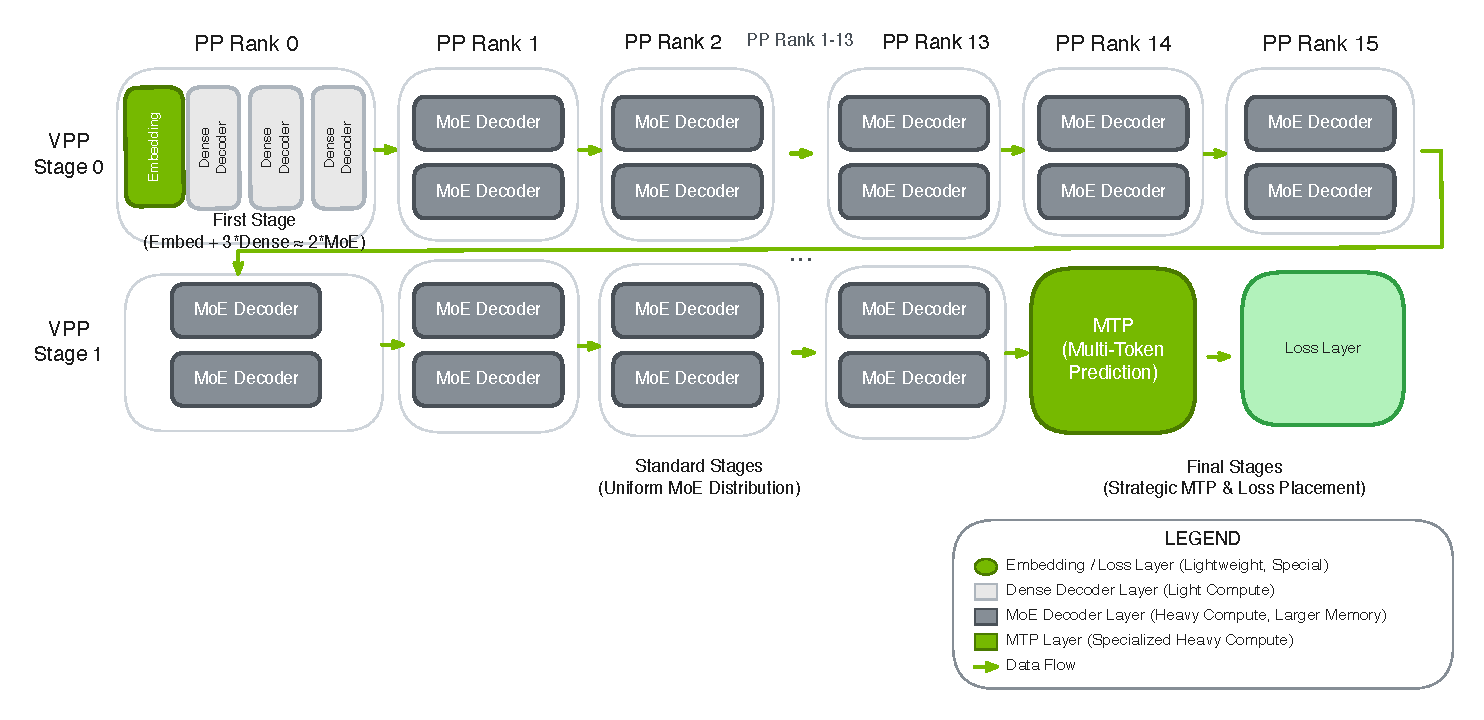
\includegraphics[width=0.95\textwidth]{figures/plots/flexible_vpp_layout_draft.pdf}
    \caption{\textbf{Flexible Pipeline Parallel Placement.}}
    \label{fig:flexible-vpp-layout}
\end{figure}

\subsection{Upcycling}
Upcycling converts a pre-trained dense model into a sparse MoE architecture, expanding model capacity without retraining from scratch~\cite{komatsuzaki2022sparse,he2024upcyclinglargelanguagemodels,vavre2024llama}. We support virtual group initialization and expert weight scaling to enable seamless adaptation of dense checkpoints into fine-grained MoE models. The approach employs softmax-then-topK routing, which routes tokens through a selective subset of experts for increased expressivity at constant or reduced inference cost, as illustrated in \figref{fig:granular_upcycling_diagram}.

\begin{figure}[!ht]
    \centering
    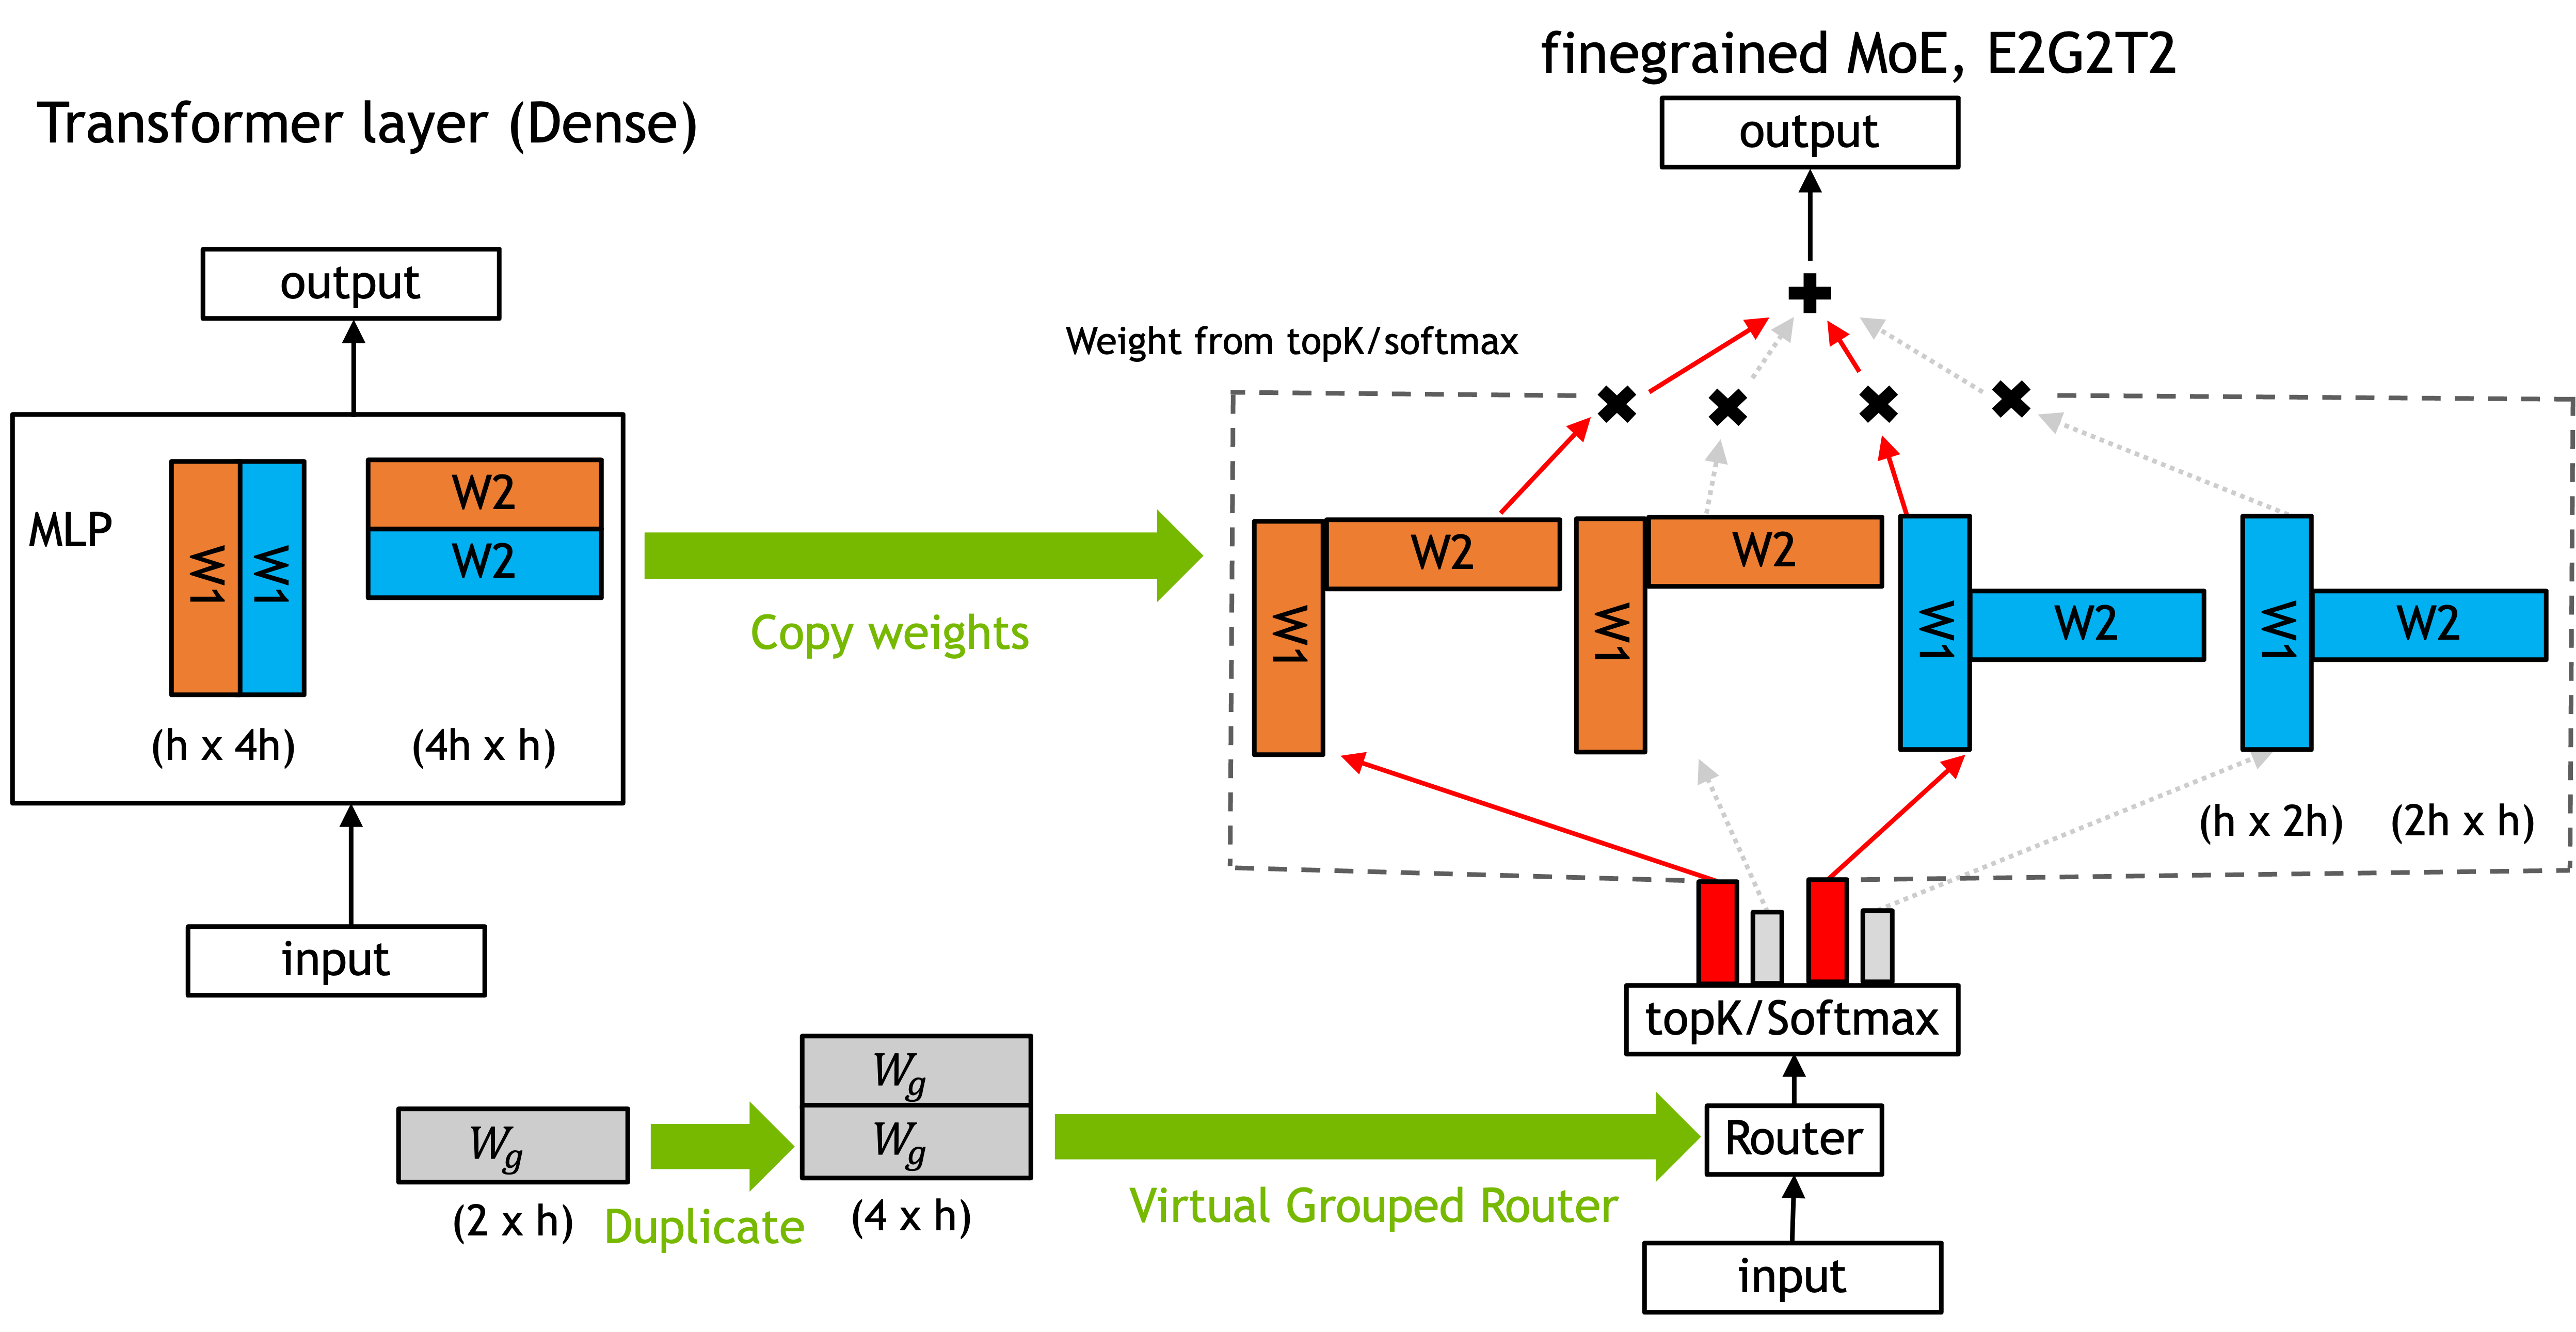
\includegraphics[width=1\textwidth]{figures/granular_upcycling.png}
    \caption{An example of granular upcycling a dense layer into E2G2T2 fine-grained MoE. E2G2T2 denotes 4 experts, top 2, with half intermediate size. (1) We shard MLP weights in the intermediate dimension ($4h \rightarrow 2h$) then duplicate the shards. (2) We initialize half the router weights then duplicate them. This ensures Top2 always selects one of each MLP shard so MoE output is the same as the dense model at the start of training.}
    \label{fig:granular_upcycling_diagram}
\end{figure}

\subsection{Multi-Token Prediction}
Multi-token prediction (MTP) optimizes a model to predict multiple consecutive future tokens at each position, densifying the supervision signal~\cite{gloeckle2024better,deepseekai2025deepseekv3technicalreport}. Unlike parallel independent predictions, MTP maintains causal dependencies between predictions through hidden state transitions, accelerating convergence and improving generation quality. During inference, the model reverts to standard single-token prediction for deployment compatibility.

We integrate MTP with flexible pipeline parallelism, allowing MTP layers to be placed strategically within the VPP layout for balanced workload distribution.

\subsection{Muon Optimizer}
Unlike traditional optimizers such as AdamW that perform element-wise updates, the Muon optimizer introduces a matrix-aware approach by orthogonalizing entire weight matrices~\cite{liu2025muonscalablellmtraining}. This improves the conditioning of optimization trajectories and significantly reduces training steps compared to AdamW.

Our integration provides production-ready support for large-scale distributed training with several key advantages: (1) full support for split query-key-value (QKV) weight layouts, enabling efficient orthogonalization even when attention projection matrices are stored as separate tensors; (2) seamless integration with the distributed optimizer, allowing optimizer states to be sharded across data-parallel ranks while maintaining correct orthogonalization semantics; and (3) CPU offloading for Muon's orthogonalization buffers when GPU memory is constrained.

\textbf{MuonClip.}
Training trillion-parameter models introduces stability challenges where query-key dot products can grow unbounded, causing attention explosions \cite{kimik2}. MuonClip addresses this with hardware-accelerated implementations in cuDNN, cudnn-frontend, and Transformer Engine.

\section{Performance Evaluation}\label{performance-evaluations}
The preceding sections described Megatron-Core MoE's architecture, parallelism strategies, and optimizations. This section validates these contributions through empirical evaluation, showing the performance of the Megatron-Core MoE stack across diverse model configurations and hardware platforms.

\begin{notebox}
\textbf{Living Document.} The performance results in this section represent a point-in-time snapshot based on Megatron-Core \textbf{v0.16}, not the upper bound of achievable performance. Active optimization efforts are ongoing, and these numbers will improve in future releases. We also plan to expand coverage to additional model architectures as they emerge in the community. For the latest performance data, please refer to the Megatron-LM and Megatron-Bridge repository.
\end{notebox}

\subsection{Experimental Setup}

\textbf{Benchmark Models.}
We evaluate Megatron-Core MoE on two state-of-the-art fine-grained MoE architectures that stress-test the framework's capabilities: DeepSeek-V3-685B~\cite{deepseekai2025deepseekv3technicalreport} and Qwen3-235B~\cite{qwen2025qwen25technicalreport,yang2025qwen3technicalreport}. Both models feature the fine-grained expert design that amplifies the Three Walls challenges: high expert counts strain memory capacity, top-k routing increases all-to-all communication volume, and smaller per-expert computations reduce GEMM efficiency. These characteristics make them demanding benchmarks for validating our optimization strategies.

\textbf{Hardware and Software Stack.}
Benchmarks are conducted on NVIDIA GB200 and H100 GPUs to assess performance across hardware generations. We use the \texttt{dev} branch of Megatron-LM\footnote{\url{https://github.com/NVIDIA/Megatron-LM/tree/dev}} with the latest TransformerEngine\footnote{\url{https://github.com/NVIDIA/TransformerEngine/tree/main}}. The full optimization stack described in Section~\ref{key-features-optimizations} is enabled, including but not limited to:
\begin{itemize}[noitemsep,topsep=0pt]
    \item \textbf{FP8 training:} MXFP8 on GB200/GB300 (Blackwell) with native Tensor Core support and blockwise FP8 on H100 (Hopper)
    \item \textbf{Memory optimizations:} Selective recomputation and activation \& optimizer state offloading to reduce peak memory footprint
    \item \textbf{Optimized token dispatchers:} HybridEP\footnote{\url{https://github.com/deepseek-ai/DeepEP/tree/hybrid-ep}} on GB200/GB300 NVL systems exploiting Multi-Node NVLink, and DeepEP\footnote{\url{https://github.com/deepseek-ai/DeepEP/tree/main}} on H100 systems
    \item \textbf{Communication overlap:} 1F1B all-to-all overlap with expert computation
    \item \textbf{Kernel optimizations:} Grouped GEMM, router fusion, permutation fusion, and CUDA Graphs
\end{itemize}

\textbf{Metrics.}
We report per-GPU throughput in TFLOPS and tokens processed per second per GPU. These metrics provide two views of computational efficiency and practical training throughput.

\subsection{Key Performance Results}


\textbf{Overview.}
Table~\ref{tab:moe_throughput_unified} summarizes per-GPU throughput for representative fine-grained MoE training workloads on NVIDIA GB300, GB200, and H100 systems under the fully enabled optimization stack described in Section~\ref{key-features-optimizations}. All configurations use force-balanced routing to ensure even token distribution across experts.

% \textbf{Mixtral-8$\times$22B (long-context stress test).}
% We additionally include Mixtral-8$\times$22B with a sequence length of 65{,}536 to highlight regimes where long-context training amplifies memory pressure and communication overhead (Table~\ref{tab:moe_throughput_unified}). At this long sequence length, FP8 training improves throughput by roughly 14\% relative to BF16 on both GB200 and H100, and the newer GB200 platform delivers substantially higher per-GPU throughput than H100.

\textbf{DeepSeek-V3 and Qwen3-235B (large-scale training).}
Table~\ref{tab:moe_throughput_unified} reports results for two contemporary, fine-grained MoE training workloads at a standard sequence length of 4{,}096, including a 1{,}024-GPU DeepSeek-V3 run on H100. Across these settings, the measurements demonstrate strong per-GPU efficiency and high sustained throughput across all three platforms.


\def\unifiedthroughputtablescale{1.1}
\begin{table}[t]
    \centering
    \caption{Unified throughput benchmarks (per-GPU figures) for two mixture-of-experts models on NVIDIA GB300, GB200, and H100. All configurations use force-balanced routing. The Dtype column specifies the FP8 recipe: FP8-BLK denotes blockwise FP8 on Hopper, and MXFP8 denotes microscaling FP8 on Blackwell.}
    \scalebox{\unifiedthroughputtablescale}{%
    \begin{tabular}{lcccccc}
    \toprule
    Model & System & \#GPUs & Seqlen & Dtype & Per-GPU TF & Tokens/s/GPU \\
    \midrule
    DeepSeek-V3   & GB300 & 256  &   4,096 & MXFP8    & 1233 & 4,730 \\
    DeepSeek-V3   & GB200 & 256  &   4,096 & MXFP8    & 1048 & 4,020 \\
    DeepSeek-V3   & GB200 & 256  &   4,096 & BF16     & 857  & 3,298 \\
    DeepSeek-V3   & H100  & 1024 &   4,096 & FP8-BLK  & 368  & 1,412 \\
    \midrule
    Qwen3-235B    & GB300 & 256  &   4,096 & MXFP8    & 974  & 6,583 \\
    Qwen3-235B    & GB200 & 256  &   4,096 & MXFP8    & 919  & 6,212 \\
    Qwen3-235B    & GB200 & 256  &   4,096 & BF16     & 750  & 5,100 \\
    Qwen3-235B    & H100  & 256  &   4,096 & BF16     & 320  & 2,132 \\
    \midrule
    Qwen3-235B    & GB300 & 128  & 131,072 & MXFP8    & 1,150  & 1,556 \\
    \bottomrule
    \end{tabular}%
    }
    \label{tab:moe_throughput_unified}
\end{table}


\textbf{FP8 Training Effectiveness.}
As shown in Table~\ref{tab:moe_throughput_unified}, FP8 training achieves 368 TFLOPS per GPU on H100 for DeepSeek-V3, demonstrating that the blockwise FP8 recipe enables efficient training of large-scale MoE models on Hopper architecture. The optimizations discussed in Section~\ref{sec:fp8-training} successfully address the challenges of applying FP8 to MoE models with dynamic expert routing and varying computation patterns, maintaining numerical stability while providing the performance benefits of reduced precision.

\textbf{GB200 and GB300 Performance.}
The GB200 and GB300 platforms deliver approximately 3$\times$ higher token throughput compared to H100 for both MoE models at comparable or smaller GPU counts. This efficiency gain stems from superior memory bandwidth, higher computational capacity, and native MXFP8 Tensor Core support. Combined with our software optimizations (Sections~\ref{sec:memory-wall} and~\ref{sec:compute-wall}), GB200 achieves over 1,048 TFLOPS per GPU for DeepSeek-V3 training, and GB300 further pushes this to 1,233 TFLOPS per GPU.

\textbf{Scalability.}
These results demonstrate that Megatron-Core MoE scales efficiently to production workloads with thousands of GPUs and hundreds of billions of parameters. The successful deployment of DeepSeek-V3 at 1,024-GPU scale validates the effectiveness of parallel folding (Section~\ref{sec:parallel-folding}), optimized dispatchers (Section~\ref{sec:comm-wall}), and kernel optimizations (Section~\ref{sec:compute-wall}).

\textbf{Long-context Stress Test).}
To capture behavior beyond the standard 4{,}096-token regime, Table~\ref{tab:moe_throughput_unified} includes a long-context Qwen3-235B run at sequence length 131{,}072 on GB300. Even in this memory- and communication-intensive setting, the system sustains 1{,}150 TFLOPS per GPU, indicating strong long-context efficiency under the full optimization stack.

\noindent
\textbf{Configuration Details.} The parallelism configurations (TP, PP, CP, EP, DP, VPP, etc.), batch settings, and other optimization details used for each benchmark entry in Table~\ref{tab:moe_throughput_unified} are provided in Appendix~\ref{sec:showcase_settings}. Note that these configurations represent our best-found settings through empirical tuning; they may not be globally optimal, as exhaustively searching the full parallelism and optimization configuration space is infeasible for models of this scale.

Section~\ref{performance-evaluations} demonstrated that Megatron-Core MoE achieves state-of-the-art performance across diverse MoE architectures on the latest GPU platforms. We now examine the systematic methodology behind these results and show how the optimizations from Sections~\ref{sec:memory-wall}--\ref{sec:compute-wall} translate into deployment decisions through detailed case studies.

\section{Performance Best Practices}\label{sec:best-practices}

Sections~\ref{parallelism-strategies}--\ref{sec:production-features} presented a comprehensive optimization arsenal for MoE training: parallel folding, optimized dispatchers, Grouped GEMM, reduced-precision training, CUDA Graphs, and more. However, \textbf{having many optimization techniques does not automatically translate into high performance}. Each technique addresses specific bottlenecks but introduces its own trade-offs. Reduced-precision training reduces memory but requires careful precision management. Communication overlap improves throughput but adds memory overhead. CUDA Graphs eliminate host latency but conflict with dynamic tensor shapes. The challenge is not the availability of optimizations; it is knowing \emph{which} optimizations to apply, \emph{when} to apply them, and \emph{how} they interact with each other.

This complexity means that achieving peak performance requires a systematic methodology, not trial-and-error tuning. Through optimization of diverse MoE models (from Mixtral to DeepSeek-V3) on GB200 and H100, we developed a repeatable workflow for identifying bottlenecks and applying targeted solutions. This section distills those lessons into actionable guidance. Section~\ref{sec:best-practices-methodology} presents the methodology under the Three Walls framework with concrete examples for each phase. Section~\ref{sec:deepseek-case-study} then shows how these principles combine for DeepSeek-V3 on GB200 and H100, including why the same model requires different strategies on different hardware.

\subsection{A Systematic Optimization Workflow}\label{sec:best-practices-methodology}

We present a three-phase workflow for MoE performance optimization. This methodology emerged from tuning Mixtral, DeepSeek-V3, and Qwen3 across GB200 and H100 platforms. The process is inherently \textbf{iterative}: solving one bottleneck often exposes the next, requiring continuous profiling and refinement.

\subsubsection{Phase 1: Establish Memory-Feasible Parallelism}

Memory feasibility is the first constraint. Before optimizing for throughput, the configuration must fit in GPU memory. Table~\ref{tab:parallel-memory-impact} summarizes how each parallelism strategy affects per-GPU memory and communication overhead.

\begin{table}[ht]
\centering
\caption{Impact of parallelism strategies on memory and communication. $d$ = parallelism degree. $^\dagger$Requires distributed optimizer (\texttt{-{}-use-distributed-optimizer}).}
\label{tab:parallel-memory-impact}
\begin{tabular}{lcccc}
\toprule
\textbf{Strategy} & \textbf{Peak Activation} & \textbf{Weight Memory} & \textbf{Optimizer States} & \textbf{Comm (Per-Layer)} \\
\midrule
TP & $1/d$ (with SP) & $1/d$ & $1/d$ & High \\
EP & $\sim$1 (load-dependent) & $1/d$ (MoE only) & $1/d$ & Medium \\
PP & 1 ($>$1 with VPP) & $1/d$ & $1/d$ & Medium \\
CP & $1/d$ & 1 & $1/d^\dagger$ & Medium \\
DP & 1 & 1 & $1/d^\dagger$ & Low \\
\bottomrule
\end{tabular}
\end{table}

\begin{notebox}
\textbf{Quick feasibility testing.} Use \texttt{-{}-fake-init-process-group} to emulate distributed training on a single GPU, enabling rapid iteration on parallelism configurations without allocating a full cluster. See the Megatron-LM documentation\footnote{\url{https://github.com/NVIDIA/Megatron-LM/pull/2254}} for detailed usage.\\
\textbf{Interactive Memory Estimator}. We have developed an interactive memory simulator with a web GUI for quick parallelism tuning against memory footprints. See the blog\cite{nvidia_memory_estimator_blog} for details.

\end{notebox}

\noindent\textbf{Example.} For a 685B-parameter fine-grained MoE model, BF16 activations alone can exceed 130\,GB per GPU (see Table~\ref{tab:memory-breakdown}), immediately ruling out baseline configurations on 80\,GB devices even with parallelism, and motivating the memory optimizations in Phase~3.

\subsubsection{Phase 2: Select Optimal Parallelism Strategy}

Once memory-feasible configurations are identified, select the strategy that minimizes communication overhead while maintaining throughput. The optimal choice depends on model architecture, sequence length, and hardware topology.

\paragraph*{Guideline 1: Minimize Model Parallelism, Maximize Data Parallelism}
\begin{itemize}
    \item \textbf{Goal:} Keep TP/EP/PP/CP as small as possible while avoiding OOM.
    \item \textbf{Why:} Model parallelism introduces communication overhead that hurts performance.
    \item \textbf{How:} Use distributed optimizer (\texttt{-{}-use-distributed-optimizer}) to shard optimizer states across DP ranks, freeing memory for larger DP size.
\end{itemize}

\paragraph*{Guideline 2: Keep EP and TP Communication Within NVLink Domain}
\begin{itemize}
    \item \textbf{Goal:} Ensure EP$\times$TP fits within the NVLink Domain (typically 8 GPUs in a single node unless Multi-Node NVLink is used).
    \item \textbf{Why:} EP and TP are communication-intensive; NVLink provides much higher bandwidth than cross-node interconnects.
    \item \textbf{Scaling:} When scaling beyond the NVLink Domain, prefer PP over expanding TP/EP across nodes.
\end{itemize}

\noindent\textbf{Note:} For very large MoE models like DeepSeek-V3, EP communication volume may exceed what NVLink can hide. In this case, enable communication-computation overlap (see Section~\ref{sec:comm-wall}) to hide EP latency behind computation.

\paragraph*{Guideline 3: Use Pipeline Parallelism (PP) for Multi-Node Scaling}
\begin{itemize}
    \item \textbf{Goal:} Use PP to distribute layers across nodes while keeping EP$\times$TP within NVLink.
    \item \textbf{VPP:} Enable Virtual Pipeline Parallelism to reduce pipeline bubbles when PP $\geq 2$.
    \item \textbf{Config:} Set \texttt{-{}-pipeline-model-parallel-layout} to control Pipeline Parallelism settings (see Section~\ref{sec:flexible-vpp}). Larger VPP usually reduces pipeline bubbles but increases P2P communications; a middle value often provides the best balance. The workloads of each VPP rank should be balanced to maximize the throughput.
\end{itemize}

\paragraph*{Guideline 4: Prefer EP over TP for Expert Layers}
EP offers several advantages over TP for MoE layers:
\begin{itemize}
    \item \textbf{Better GEMM efficiency:} Larger local matrix sizes improve GPU utilization.
    \item \textbf{Lower communication:} EP has less communication overhead than TP for MoE layers.
    \item \textbf{Simpler computation graph:} Easier to overlap communication with computation.
    \item \textbf{Token permutation:} When EP $=$ \texttt{num\_experts}, local token permutation is eliminated.
\end{itemize}

\noindent\textbf{Example:} For Mixtral-8$\times$7B, EP8$\times$TP1 outperforms EP4$\times$TP2.

\paragraph*{Guideline 5: Enable Context Parallelism (CP) for Long Sequences}
\begin{itemize}
    \item \textbf{When to use:} Sequence length $\geq$ 8K tokens.
    \item \textbf{When to avoid:} For sequences $<$ 4K tokens, CP overhead typically exceeds benefits.
    \item \textbf{Key factor:} CP efficiency depends on overlapping communication with computation.
    \item \textbf{Config:} Set \texttt{-{}-context-parallel-size} to partition sequences across GPUs.
\end{itemize}

\noindent\textbf{Example.} Consider a 256-expert MoE model on an NVL72 system. Applying Guideline~4, Parallel Folding sets expert TP\,=\,1 so that each expert runs on a single GPU, maximizing GEMM efficiency. With Guideline~2, EP64 fits entirely within the NVLink domain. Guideline~1 then drives the remaining choices: the available memory budget determines TP and PP for attention layers, with DP filling the rest.

\subsubsection{Phase 3: Profile and Optimize Bottlenecks}

With a working parallelism configuration established, profile the training run to identify which wall dominates. Apply targeted optimizations based on the bottleneck type.

\paragraph*{Memory Bottleneck (Memory Wall)}
\textbf{Symptom:} Forced to use full recomputation or excessively large parallelism degrees to avoid OOM.

\noindent\textbf{Solutions:} Apply memory-saving techniques (Table~\ref{tab:memory-bottleneck}) to reduce memory consumption.

\begin{table}[ht]
\centering
\caption{Memory bottleneck solutions.}
\label{tab:memory-bottleneck}
\resizebox{\textwidth}{!}{%
\begin{tabular}{llll}
\toprule
\textbf{Optimization} & \textbf{Overhead} & \textbf{Config} & \textbf{Reference} \\
\midrule
FP8 Training & Low & \texttt{-{}-fp8-format -{}-fp8-recipe} & \S\ref{sec:fp8-activation} \\
Selective Recomputation & Low & \texttt{-{}-recompute-granularity -{}-recompute-modules} & \S\ref{sec:recomputation} \\
Precision-Aware Optimizer & Low & \texttt{-{}-use-precision-aware-optimizer} & \S\ref{sec:precision-opt} \\
Activation Offloading & Medium & \texttt{-{}-fine-grained-activation-offloading -{}-offload-modules} & \S\ref{sec:offloading} \\
Optimizer Offloading & Medium & \texttt{-{}-offload-optimizer-states} & \S\ref{sec:precision-opt} \\
\bottomrule
\end{tabular}%
}
\end{table}

\paragraph*{Communication Bottleneck (Communication Wall)}
\textbf{Symptom:} Profiling shows significant time spent in collective operations.

\noindent\textbf{Solutions:} Identify which communication is the bottleneck and apply the corresponding optimization. (Table~\ref{tab:comm-bottleneck})

\begin{table}[ht]
\centering
\caption{Communication bottleneck solutions.}
\label{tab:comm-bottleneck}
\resizebox{\textwidth}{!}{%
\begin{tabular}{lll}
\toprule
\textbf{Communication Type} & \textbf{Config} & \textbf{Reference} \\
\midrule
DP gradient reduce and param gather & \texttt{-{}-overlap-grad-reduce -{}-overlap-param-gather} & --- \\
TP communication & \texttt{-{}-tp-comm-overlap} & --- \\
EP dispatcher & \texttt{-{}-moe-token-dispatcher-type} & \S\ref{sec:deepep} \\
EP all-to-all hiding & \texttt{-{}-overlap-moe-expert-parallel-comm} & \S\ref{sec:comm-overlap} \\
PP send/recv & \texttt{-{}-pipeline-model-parallel-layout} & \S\ref{sec:flexible-vpp} \\
\bottomrule
\end{tabular}%
}
\end{table}

\paragraph*{CPU Overhead Bottleneck (Compute Efficiency Wall)}
The Compute Efficiency Wall manifests in two distinct forms: CPU overhead and computation inefficiency. CPU overhead occurs when the host cannot launch GPU kernels fast enough, creating gaps in GPU execution.

\noindent\textbf{Symptom:} Nsight Systems timeline shows gaps between GPU kernels where CPU cannot launch kernels fast enough.

\noindent\textbf{Solutions:} Reduce host-side overhead by minimizing kernel launches and enabling CUDA Graphs (Table~\ref{tab:cpu-bottleneck}).

\begin{table}[ht]
\centering
\caption{CPU overhead bottleneck solutions.}
\label{tab:cpu-bottleneck}
\begin{tabular}{lll}
\toprule
\textbf{Optimization} & \textbf{Config} & \textbf{Reference} \\
\midrule
Disable Python GC & \texttt{-{}-manual-gc -{}-manual-gc-interval 10} & --- \\
Reduce kernel launches & Decrease TP or increase MBS & --- \\
Enable CUDA Graphs & \texttt{-{}-cuda-graph-impl transformer\_engine} & \S\ref{sec:cuda-graphs} \\
\bottomrule
\end{tabular}
\end{table}

\paragraph*{Computation Bottleneck (Compute Efficiency Wall)}
Computation inefficiency occurs when GPU kernels themselves underutilize hardware resources, typically due to small GEMM sizes in fine-grained MoE architectures.

\noindent\textbf{Symptom:} GPU SM utilization is low despite no communication or CPU bottlenecks.

\noindent\textbf{Solutions:} Improve kernel efficiency through batching, fusion, and lower precision (Table~\ref{tab:compute-bottleneck}).

\begin{table}[ht]
\centering
\caption{Computation bottleneck solutions.}
\label{tab:compute-bottleneck}
\begin{tabular}{llp{4cm}}
\toprule
\textbf{Optimization} & \textbf{Config} & \textbf{Reference} \\
\midrule
Grouped GEMM & \texttt{-{}-moe-grouped-gemm} & \S\ref{sec:kernel-fusion} \\
Kernel fusions & \texttt{-{}-moe-router-fusion -{}-moe-permute-fusion} & \S\ref{sec:kernel-fusion} \\
FP8 precision & \texttt{-{}-fp8-format -{}-fp8-recipe} & \S\ref{sec:reduced-precision-training} \\
\bottomrule
\end{tabular}
\end{table}

\noindent\textbf{Example.} On an NVL8 system where EP spans across nodes, profiling may reveal all-to-all communication consuming 30--50\% of step time, pointing squarely at the Communication Wall. On an NVL72 system where the same EP degree stays within the NVLink domain, the dominant bottleneck after enabling FP8 often shifts to CPU overhead instead; the faster GPU computation exposes host-side launch latency. The same model on different hardware can require entirely different optimization strategies.

\subsubsection{Summary}

The ordering of the three phases matters: memory constraints are a hard barrier that must be resolved first (Phase~1), parallelism decisions determine the communication topology (Phase~2), and only then can profiling reveal which wall to attack (Phase~3). Crucially, this process is \textbf{iterative}. Memory optimizations may enable smaller parallelism degrees, returning to Phase~1. Some Phase~3 optimizations have their own memory cost (EP communication overlap requires extra buffers, CUDA Graphs consume additional memory), which may require revisiting earlier decisions. Continuous profiling after each round guides the next iteration.

\subsection{Case Study: Tuning DeepSeek-V3 on GB200 and H100}\label{sec:deepseek-case-study}

DeepSeek-V3 represents an extreme stress test for MoE training: 685B total parameters with Multi-Token Prediction (MTP) and Multi-Latent Attention (MLA). All three walls apply: memory pressure from 256 experts, high all-to-all volume from top-8 routing, and small per-expert GEMMs. The preceding workflow (Section~\ref{sec:best-practices-methodology}) showed how to approach each phase individually; this case study examines how those decisions interact to form a coherent optimization stack, and why the same model requires fundamentally different strategies on GB200 and H100.

\subsubsection{Final Optimized Configuration and Performance}

Table~\ref{tab:deepseekv3-config} summarizes the final optimized configurations and performance on GB200 and H100 platforms.

\begin{table}[ht]
\centering
\caption{DeepSeek-V3 final optimized configurations on GB200 and H100. $^\dagger$Parallel Folding is used; TP applies to the non-MoE modules only, expert TP is always 1.}
\label{tab:deepseekv3-config}
\begin{tabular}{lcc}
\toprule
\textbf{Configuration} & \textbf{GB200} & \textbf{H100} \\
\midrule
Hardware & 256$\times$GB200 & 1024$\times$H100 \\
Parallelism (TP/PP/EP)$^\dagger$ & 1/4/64 & 2/8/64 \\
VPP & 4 & 4 \\
GBS / MBS / SeqLen & 8192 / 1 / 4096 & 8192 / 1 / 4096 \\
Precision & MXFP8 & FP8-Blockwise \\
Dispatcher & HybridEP & DeepEP \\
Recompute & \texttt{mlp} & \texttt{mlp}, \texttt{mla\_up\_proj}, \texttt{moe\_act}, \texttt{layernorm} \\
CUDA Graphs & Enabled & --- \\
EP all-to-all Overlap & --- & Enabled \\
\midrule
\textbf{Performance (TFLOPS/GPU)} & \textbf{1048} & \textbf{368} \\
\bottomrule
\end{tabular}
\end{table}

The GB200 configuration uses HybridEP (optimized for NVL72) and CUDA Graphs to minimize CPU overhead, which becomes the dominant bottleneck in FP8 training on Blackwell. The H100 configuration uses FP8-blockwise precision with DeepEP and EP all-to-all overlap to hide communication latency.

Table~\ref{tab:deepseekv3-journey} summarizes the key optimizations applied on each platform.

\begin{table}[ht]
\centering
\caption{DeepSeek-V3 optimization summary by platform.}
\label{tab:deepseekv3-journey}
\begin{tabular}{lp{5cm}p{5cm}}
\toprule
\textbf{Category} & \textbf{GB200} & \textbf{H100} \\
\midrule
Parallelism & Parallel Folding \newline Flexible VPP & Parallel Folding \newline Flexible VPP \\
\midrule
Precision & MXFP8 & FP8-Blockwise \\
\midrule
Memory & Memory-efficient permutation \newline Fine-grained recomputation \newline FP8 primary weights \newline Low-precision optimizer states \newline Optimizer states offloading & Memory-efficient permutation \newline Fine-grained recomputation \newline FP8 primary weights \newline Low-precision optimizer states \\
\midrule
Communication & HybridEP & DeepEP \newline EP Communication overlap \\
\midrule
Compute Efficiency & Kernel fusions \newline CUDA Graphs \newline CPU-side optimizations & Kernel fusions \\
\bottomrule
\end{tabular}
\end{table}

\subsubsection{Anatomy of the Optimized Configuration}

\paragraph*{Why This Parallelism Layout?}
Both platforms use Parallel Folding (Guideline~4) to decouple attention and expert parallelism: TP applies only to attention layers for memory reduction, while experts use EP with TP\,=\,1 for better GEMM efficiency. EP64 is chosen so that each GPU holds exactly four of the 256 experts, eliminating local token permutation overhead.

The key platform difference is memory capacity. GB200's 192\,GB per GPU (vs.\ H100's 80\,GB) allows TP1/PP4 instead of TP2/PP8, halving the pipeline depth, which reduces pipeline bubbles and simplifies workload balancing (Guideline~1). Flexible VPP then fine-tunes the pipeline: on H100, the layout \texttt{Et*3|(tt|)*29m|L} groups embedding with 3 transformer layers in the first stage, places MTP in a standalone stage, and separates the loss; on GB200, \texttt{Et*4|(tttt|)*14tmL} distributes layers across 16 virtual stages for balanced computation across the shorter pipeline. These parallelism configurations establish the foundation for all subsequent optimizations.

\paragraph*{Memory Wall}
FP8 training is the first lever: it halves activation memory on both platforms, freeing GPU memory that would otherwise require aggressive recomputation. On H100, the freed memory budget is critical because it enables EP communication overlap, which requires extra buffers for pipelining dispatch and combine operations (see Communication Wall below). Fine-grained recomputation (\texttt{mlp}, \texttt{mla\_up\_proj}, \texttt{layernorm}, \texttt{moe\_act}) trims remaining memory pressure. Memory-efficient permutation eliminates redundant activation storage, and low-precision optimizer states (BF16) provide additional headroom.

On GB200, the memory chain resolves differently. NVL72 keeps EP local, so communication overlap is not critical and its memory budget is freed entirely. GB200's higher C2C bandwidth (NVLink-C2C) makes optimizer state offloading effective: the transfer overhead is low enough that offloading frees substantial GPU memory for activations. This in turn reduces the need for fine-grained recomputation to just \texttt{mlp}, far less aggressive than on H100.

\paragraph*{Communication Wall}
On H100/B200 (NVL8), EP64 spans 8 nodes, and cross-node all-to-all latency would consume nearly 50\% of step time with the standard all-to-all dispatcher. DeepEP reduces this overhead through fused permutation and optimized collective operations. Even so, EP communication overlap is essential to hide the remaining cross-node latency behind expert computation, and this overlap is only feasible because FP8 freed enough memory for the extra buffers (see Memory Wall above).

On GB200 (NVL72), EP64 stays entirely within the NVLink domain. HybridEP fully utilizes the 1.8\,TB/s bidirectional bandwidth without requiring communication overlap. The communication wall is effectively resolved by hardware topology alone, shifting the dominant bottleneck to compute efficiency.

\paragraph*{Compute Efficiency Wall}
FP8 accelerates GEMMs on both platforms (blockwise FP8 on H100, MXFP8 with native Blackwell Tensor Core support on GB200), but this speedup has a side effect: faster GPU computation exposes CPU overhead. On GB200, where NVL72 already eliminates the communication bottleneck, CPU overhead becomes the dominant constraint; the host cannot launch kernels fast enough to keep the GPU saturated.

Partial CUDA Graphs address this by capturing attention, router, and MoE preprocessing into static graphs, while leaving dynamic expert computation ungraphed. Kernel fusions (router fusion, permute fusion, MLA RoPE fusion) reduce kernel launch count. CPU/NUMA binding\footnote{The \texttt{bindpcie} script at \url{https://github.com/NVIDIA/mlperf-common/blob/main/client/bindpcie} automatically detects GPU/NUMA topology based on local rank and uses \texttt{numactl} to bind each process's CPU and memory to the NUMA node nearest its GPU.} reduces host-side memory access latency.

\medskip

The cross-cutting nature of these optimizations is evident throughout: FP8 simultaneously reduces memory (activations halved), and improves compute throughput, but introduces quantization kernels that amplify CPU overhead. The same model arrives at fundamentally different optimization stacks on different hardware: H100's stack centers on hiding communication latency (DeepEP + EP overlap), while GB200's centers on eliminating CPU overhead (CUDA Graphs + kernel fusions). This contrast validates the profile-driven iterative approach from Section~\ref{sec:best-practices-methodology}.

\subsubsection{Lessons Learned}

Four insights generalize beyond DeepSeek-V3:

\begin{enumerate}
    \item \textbf{Platform characteristics drive strategy}: GB200's larger memory (192GB vs 80GB) and higher C2C bandwidth enable more aggressive choices: smaller PP degree, less fine-grained recomputation, and effective optimizer offloading. H100's NVL8 requires EP communication overlap to hide cross-node latency, while GB200's NVL72 keeps EP64 within the NVLink domain.
    \item \textbf{Parallel Folding unlocks flexibility}: Decoupling attention TP from expert EP allows independent optimization of each layer type. Combined with flexible VPP, this enables fine-grained workload balancing across pipeline stages.
    \item \textbf{FP8 shifts bottlenecks}: FP8 training accelerates GEMMs and reduces memory, but amplifies CPU overhead as the dominant bottleneck. CUDA Graphs, kernel fusions, and CPU/NUMA binding become essential.
    \item \textbf{Iterative optimization}: The optimization process is inherently cyclical. Memory optimizations (recomputation, offloading) free GPU memory, enabling communication overlap. Communication optimizations expose compute efficiency bottlenecks. Some optimizations have cross-cutting effects: FP8 training reduces both memory and compute time but increases CPU overhead; CUDA Graphs reduce CPU overhead but consume additional memory. These interactions mean that applying one optimization may require revisiting earlier decisions. Continuous profiling after each change guides the next optimization target and helps identify when diminishing returns suggest moving to the next bottleneck.
\end{enumerate}

